\documentclass[12pt, a4paper]{article}
\usepackage[T1]{fontenc}
\usepackage[utf8]{inputenc}
\usepackage[french]{babel}
\usepackage{geometry}
\usepackage{graphicx}
\usepackage{wrapfig}
\usepackage{indentfirst}
\usepackage{tikz}
\usepackage{igo}

\graphicspath{{/home/pgi/TIPE/content/Rapport/image/}}
\usetikzlibrary{trees}

% Title
\title{Rapport de TIPE\\
Morpion}
\author{Peng-Wei Chen, MP, \oldstylenums{2017}-\oldstylenums{2018}}

\begin{document}

\maketitle
\tikzstyle{point}=[circle,draw,thin,fill=white]

\section{Introduction}
\subsection{La règle du morpion}
Deux joueurs jouent sur une grille de taille $15 \times 15$ sur le papier. Chaqu'un prend un symbole et on dessine au tour par tour son symbole sur la grille. Le but est d'aligner 5 symboles verticalement, horizontalement ou en diagonale pour gagner.
Dans le cas généralisé, nous appelons (m, n, k)-jeu où la taille de la grille est $m \times n$ et il faut $k$ symboles dans une ligne pour gagner.
\subsection{Méthode}
Il existe deux méthodes pour déterminer s'il existe une telle stratégie:
\begin{itemize}
    \item On cherche tous les cas possibles.
    \item On apparie les points de la grille. Si le deuxième joueur peut toujours prévenir la réussite du premier joueur en jouant le pairage, alors il n'y a pas d'une telle stratégie.
\end{itemize}

Dans le cas où k $\le$ 7, on utilise la première méthode avec l'arbre de décision. Chaque nœud de cet arbre est un état de la grille. Par exemple (figure. \ref{fig:arbre}) , la racine de cet arbre est la grille sans symbole. Ensuite, les fils de chaque nœud sont les états de la grille où on place un symbole de plus au dessus. Enfin, les feuilles sont les cas où un des joueurs a gagné ou où personne n'a gagné (c'est-à-dire que la grille a été remplie et que aucun joueur a aligné k symboles).

\begin{figure}[t]
\centering
\gobansize{3}
\black{b2}
\copytogoban{2}
\white{a3}
\copytogoban{3}
\clear{a3}
\white{a2}
\copytogoban{4}
\cleargoban
\black{a2}
\copytogoban{5}
\clear{a2}
\black{a3}
\copytogoban{6}
\clear{a3}

\begin{tikzpicture}[level distance=2cm,
    level 1/.style={sibling distance=4cm},
level 2/.style={sibling distance=1.5cm}]
  \node {\showfullgoban}
  child {node {\usegoban{2} \showfullgoban}
      child {node {\usegoban{3} \showfullgoban}
      child {node {$\vdots$}}}
      child {node {\usegoban{4} \showfullgoban}
      child {node {$\vdots$}}}
    }
    child {node {\usegoban{5} \showfullgoban}
        child {node {$\vdots$}}
        child {node {$\vdots$}}
    }
    child {node {\usegoban{6} \showfullgoban}
        child {node {$\vdots$}}
        child {node {$\vdots$}}
    };
\end{tikzpicture}
\caption{Arbre de décision (le cercle noir est le symbole du premier joueur)} \label{fig:arbre}
\end{figure}

Or, la complexité de chercher tous les cas possibles est en O(($m \times n$)!). Ainsi, on utilise une fonction gloutonne pour chercher le cas le \og plus \fg possible. Avec cette fonction, on donne une note à chaque point. Si un point est plus possible pour gagner, alors sa note est plus élevée.\par
On utilise la deuxième méthode lorsque k > 7.

\section{Exploitation}
\subsection{k $\le$ 5}
Afin de diminuer la complexité, on essaie de créer une fonction qui a l'état de la grille comme entrée et renvoie les meilleurs positions. Ainsi, à chaque nœud de l'arbre de décision, on a diminué le nombre des cas possibles - tous les positions à un certain nombre de positions possibles.
\subsubsection{Fonction naïve}
L'idée est simple: on considère le nombre de symboles non séparés dans une ligne. Par exemple (Exemple 1), s'il y a trois symboles dans une ligne, on donne une note de 81 ($3^{4}$) au point où on aura quatre symboles dans une ligne (les triangles).
\gobansize{10}
\black{d5,e5,f5}
\white[\igotriangle]{c5,g5}
\begin{center}
    \shortstack{\showgoban\\Exemple 1}
\end{center}
Il y a deux cas possibles, qu'on appelle i-vivre ou i-mort où i est le nombre de symboles déjà aligné, vivre si les deux cotés sont libres, mort si seul un des deux coté est libre. Si les deux cotés ne sont pas libres, alors la note vaut 0 (impossible de compléter en k symboles dans la même ligne).
\clear{c5,g5}
\begin{center}
    \shortstack{\showgoban\\3-vivre}
    \white{g5}
    \shortstack{\showgoban\\3-mort}
\end{center}
\begin{center}
    \white{c5}
    \shortstack{\showgoban\\La note est nulle}
\end{center}
Dans notre fonction, on donne $3^{i}$ au cas de i-vivre et $3^{i-1}$ au celui de i-mort car j-mort est en effet le cas de (j$+$1)-vivre. En particulier, on donne $3^{k+1}$ au cas où le premier joueur est sûrement gagné, c'est-à-dire k-mort ou (k-1)-vivre. En même temps, il faut considérer les quatre directions. Par exemple (Exemple 2), si k $=$ 5, le cas 4-mort-4-mort est un cas gagnant (le deuxième joueur ne peut que prévenir la réussite d'une direction, les deux x).
\cleargoban
\begin{center}
    \black{d5,e5,f5,g3,g4,g6}
    \white{c5,g7}
    \white[\igotriangle]{g5}
    \gobansymbol{h5,g2}{x}
    \shortstack{\showgoban\\Exemple 2}
\end{center}
On a ainsi une fonction naïve.

\subsubsection{Améliorer notre fonction avec l'élagage alpha-beta}
Dans notre fonction, on ne considère que l'état de la grille, et elle n'est pas correcte dans certains cas. Par exemple \mbox{(Exemple 3.1)}, au début du jeu, le premier joueur place son symbole au centre de la grille. Ensuite, le deuxième joueur place en haut à gauche du centre. Dans ce cas-là, la fonction renvoie 6 positions (3.2) avec la même note. Cependant, l'une de ces positions donne l'avantage au deuxième joueur. (3.3) Dans ce cas-là, le deuxième joueur peut défendre et essayer d'aligner ses symboles en même temps. 
\begin{center}
    \cleargoban
    \gobansize{5}
    \black[1]{c3}
    \white[2]{b4}
    \shortstack{\showfullgoban\\1}
    \cleargoban
    \black{c3}
    \white{b4}
    \white[\igotriangle]{b3,b2,c2,c4,d3,d4}
    \shortstack{\showfullgoban\\2}
    \cleargoban
    \black{c3,d3}
    \white{b4}
    \white[\igotriangle]{b3}
    \shortstack{\showfullgoban\\3}
    \\
    Exemple 3
\end{center}
\par
On utilise l'arbre de décision pour améliorer notre fonction, de sorte que notre fonction \og pense\fg \ à l'étape d'après. Pour le faire, on utilise l'algorithme de minimax. Dans cet algorithme, on utilise notre fonction naïve et la note est calculée par la difference de celle du premier joueur et celle du deuxième joueur. Cette note peut être eventuellement négative. Ainsi, dans le niveau du premier joueur (niveau max), on veux que la note soit plus élevée tandis que la note est plus faible dans le niveau du deuxième joueur (niveau min).

%% minimax
\begin{tikzpicture}[level distance=2cm,
    level 1/.style={sibling distance=4cm},
level 2/.style={sibling distance=4cm},
level 3/.style={sibling distance=1.5cm}]
\node (n){$\circ$}
  child {node (n0){27}
      child {node (n1){27}
          child {node {4}}
          child {node (n2){27}}
          child {node {13}}
      }
      child {node (n3){29}
          child {node {2}}
          child {node {23}}
          child {node (n4){29}}
      }
    }
    child {node (n5){$\circ$}
        child {node (n6){$\vdots$}}
    };
    \node[right of=n5,node distance=4cm] {max};
    \node[right of=n6,node distance=4cm] {min};
    \node[right of=n4,node distance=4.5cm] {max};
    \node[right of=n,node distance=6cm] {Origine};
    \draw[->,draw=red] (n2) -- (n1);
    \draw[->,draw=red] (n4) -- (n3);
    \draw[->,draw=red] (n1) -- (n0)
    ;
\end{tikzpicture}

%alpha-beta
Dans l'arbre de décision, on donne la note de la position si c'est une feuille. Lorsqu'on est dans un nœud du niveau max (resp. min), on compare les notes de ses fils et en choisit la plus grande (resp. petite). En pratique, on se donne une hauteur et on fait un parcours en profondeur.\par
On peut encore améliorer cet algorithme en utilisant l'algorithme de l'élagage alpha-beta. Dans l'algorithme de minimax, on peut couper les arêtes dans certains cas. Par exemple, dans le niveau max, on a déjà déterminé la note d'un nœud 81. Or dans le nœud A, sa note est donnée par le minimum du niveau prochain. Ainsi, dans le niveau prochain, on peut s'arrêter dès qu'on a une note inférieure à 81. On appelle coupure alpha (resp. coupure beta) lorsqu'on est dans le niveau max (resp. niveau min) et une des notes des fils d'un nœud est inférieure (resp. supérieure) à celle de son frère.
\begin{tikzpicture}
%%alpha
    \node[point] (n0){\ }
    child {node {81}}
    child {node[point] (n1){A}
        child {node (n2){105}}
        child {node (n3){41}}
    }
    ;
    \node[right of=n1,node distance=2cm] {max};
    \node[right of=n3,node distance=1.3cm] {min};
    \node[below of=n2] {Coupure alpha};
    \draw[-] (n3) to node{X} (n1);
    \draw[-] (n1) to node{X} (n0);
%%beta
    \node[point,right of=n0,node distance=7cm] (n){\ }
    child {node {40}}
    child {node[point] (n4){\ }
        child {node (n5){35}}
        child {node (n6){77}}
    }
    ;
    \node[right of=n4,node distance=2cm] {min};
    \node[right of=n6,node distance=1.3cm] {max};
    \node[below of=n5] {Coupure beta};
    \draw[-] (n6) to node{X} (n4);
    \draw[-] (n4) to node{X} (n);


\end{tikzpicture}

On utilise la fonction améliorée pour chercher la stratégie gagnante du premier joueur.

\subsection{k $\ge$ 8}
En effet, si on peut montrer que le premier joueur n'a pas de stratégie gagnante lorsque k = 8, alors le premier joueur n'en a pas pour tout k $\ge$ 8 car la même stratégie du deuxième joueur parvient le premier à aligner 8 symboles. On donne notamment le pairage du cas k = 9 \mbox{(figure. \ref{fig:m-n-9})} car il est plus intuitif.
\begin{figure}[h!]
    \centering
    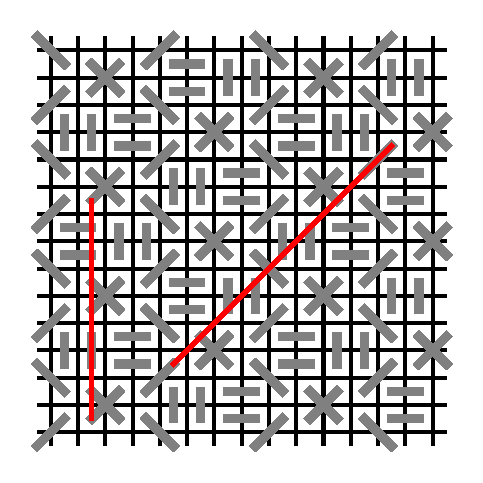
\includegraphics{m-n-9.eps}
    \caption{(m, n, 9)-jeu}
    \label{fig:m-n-9}
\end{figure}
On voit que si le deuxième joueur suit le pairage, alors le premier joueur ne peut jamais réussir (les lignes rouges).\\
Lorsque k = 8, on divise le jeu en des sous-jeux. Ces sous-jeux se jouent sur la grille de la forme comme \mbox{figure. \ref{fig:sous-jeu}.}
\begin{figure}[h!]
    \centering
    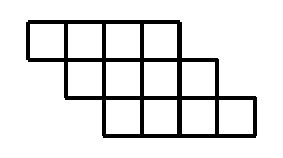
\includegraphics{m-n-8-little.eps}
    \caption{La grille du sous-jeu}
    \label{fig:sous-jeu}
\end{figure}
Il y a trois façons de gagner ce sous-jeu \mbox{(figure. \ref{fig:regle}):}
\begin{itemize}
    \item Aligner trois symboles en diagonale.
    \item Aligner verticalement deux symboles.
    \item Aligner horizontalement quatre symboles.
\end{itemize}
\begin{figure}[h!]
    \centering
    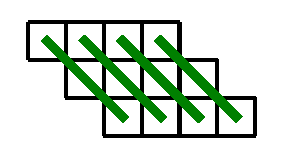
\includegraphics{8-rules1.eps}
    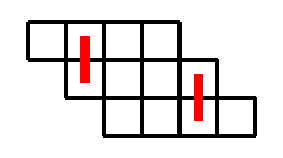
\includegraphics{8-rules2.eps}
    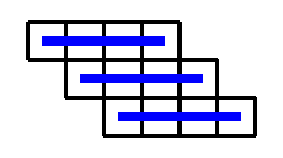
\includegraphics{8-rules3.eps}
    \caption{Les trois façons pour gagner le sous-jeu.}
    \label{fig:regle}
\end{figure}
Ainsi, puisque le premièr joueur ne peut jamais gagner ce sous-jeu, il ne peut pas non plus gagner le (m, n, 8)-jeu. (figure. \ref{fig:m-n-8})
\begin{figure}[h!]
    \centering
    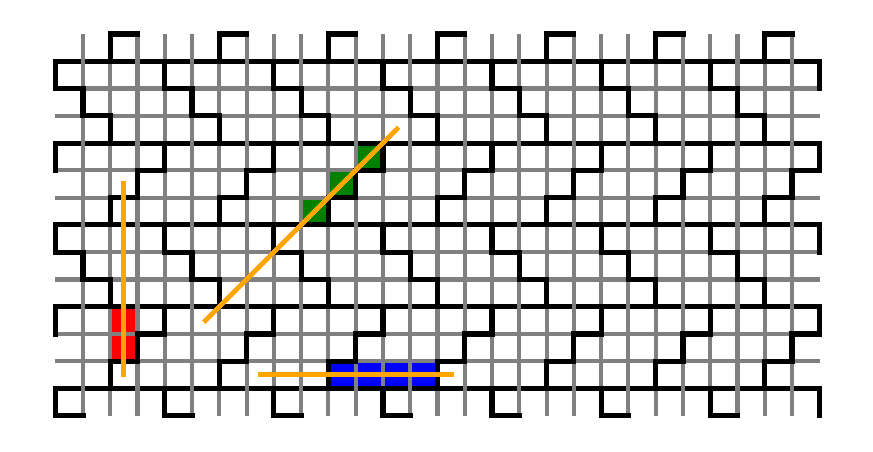
\includegraphics{8-sol.eps}
    \caption{(m, n, 8)-jeu:
    toutes les lignes de longueur 8 passent une des lignes du sous-jeu.}
    \label{fig:m-n-8}
\end{figure}
\section{Conclusion}

\begin{itemize}
    \item k = 3
    \item k = 4
    \item k = 5
    \item k $\ge$ 8\\
        Une telle stratégie n'existe pas.
\end{itemize}


\end{document}
